\documentclass[a4paper,10pt]{book}
\usepackage[utf8]{inputenc}
%\usepackage{babel}
\usepackage{verbatim} %for å inkludere filer med tegn LaTeX ikke liker
\usepackage[document]{ragged2e}
\bibliographystyle{plain}
\usepackage{amsmath}
\usepackage[pdftex]{graphicx}
\usepackage{textcomp}
\usepackage{float}
\usepackage{hyperref}
\usepackage[top=0.6in, bottom=0.8in, left=0.9in, right=0.7in]{geometry}
\usepackage{listings}
\usepackage{color}
\usepackage{tikz}
\usepackage{booktabs} 

\begin{document}

\definecolor{codegreen}{rgb}{0,0.6,0}
\definecolor{codegray}{rgb}{0.5,0.5,0.5}
\definecolor{codepurple}{rgb}{0.58,0,0.82}
\definecolor{backcolour}{rgb}{0.95,0.95,0.92}
 
\lstdefinestyle{mystyle}{
    backgroundcolor=\color{backcolour},   
    commentstyle=\color{codegreen},
    keywordstyle=\color{magenta},
    numberstyle=\tiny\color{codegray},
    stringstyle=\color{codepurple},
    basicstyle=\footnotesize,
    breakatwhitespace=false,         
    breaklines=true,                 
    captionpos=b,                    
    keepspaces=true,                 
    numbers=left,                    
    numbersep=5pt,                  
    showspaces=false,                
    showstringspaces=false,
    showtabs=false,                  
    tabsize=2
}
 
\lstset{style=mystyle}


\section*{Flat plate integral analysis}
We have the following velocity profile:
\begin{align}
u = U \sin (\frac{\pi y}{2 \delta}) \label{u}
\end{align}

To check for how realistic this velocity profile is, we have to check which boundary conditions that will be 
fulfilled with this profile.\\

\begin{align}
u(0) &= U \sin(0) = 0 \label{BC1}\\
u(\delta) &= U \sin (\frac{\pi}{2}) = U \label{BC2}\\ \nonumber \\
\frac{d u}{d y} \bigg\rvert_{y=\delta} &= \frac{\pi}{2 \delta} U \cos(\frac{\pi}{2}) = 0 \label{BC3}\\ \nonumber \\
\frac{d^2 u}{d y^2} \bigg\rvert_{y=0} &= -\frac{\pi^2}{4 \delta^2} U \sin(0) = 0 \label{BC4}\\ \nonumber
\end{align}
We can conclude that this sinus shaped velocity profile is a more realistic profile than the quadratic one\\ 
((4-11) in the book), since this velocity profile also satisfies the zero pressure-gradiet condition (\ref{BC4}), 
whereas the parabolic velocity profile only satisfies (\ref{BC1}) - (\ref{BC3}).\\
\vspace{4mm}
For the momentum thickness we have:
\begin{align}
\begin{split}
\theta &= \int_0^\delta \frac{u}{U}(1- \frac{u}{U}) dy 
= \delta \int_0^1 \frac{u}{U}(1- \frac{u}{U}) d\eta \quad,\quad 
\text{ where: } \eta = \frac{y}{\delta}\\
\theta &= \delta \int_0^1 \sin (\frac{\pi}{2} \eta) (1- \sin(\frac{\pi}{2} \eta)) d \eta\\
&= \delta \int_0^1 (\sin (\frac{\pi}{2} \eta) - \sin^2(\frac{\pi}{2} \eta)) d \eta\\
&= \delta \Big[ -\frac{2}{\pi} cos(\frac{\pi}{2} \eta) - 
\frac{\eta}{2} + \frac{1}{2 \pi} \sin(\pi \eta) \Big]_0^1\\
&= \delta (-\frac{1}{2} + \frac{2}{\pi}) = \frac{4 - \pi}{2 \pi} \delta = 0.1366 \hspace{1mm} \delta \label{theta}
\end{split}
\end{align}

Displacement thickness:
\begin{align}
\delta^* &= \int_0^\delta (1- \frac{u}{U}) dy = \int_0^\delta (1-\sin(\frac{\pi y}{2 \delta})) dy \label{deltastar1}
\end{align}

\begin{align*}
y &= \eta \delta \quad,\quad dy = \delta d \eta\\
y &= 0 \Rightarrow \eta = 0\\
y &= \delta \Rightarrow \eta = 1
\end{align*}

\begin{align}
\begin{split}
\Longrightarrow \delta^* &= \delta \int_0^1 (1- \sin(\frac{\pi}{2} \eta)) d \eta
= \Big[ \eta + \frac{2}{\pi} \cos (\frac{\pi}{2}) \Big]_0^1
= \delta (1- \frac{2}{\pi}) = 0.3634 \hspace{1mm} \delta \label{deltastar2}
\end{split}
\end{align}

For the friction coefficient we have:\\
\begin{align}
C_f &= \frac{t \tau _w}{\rho U^2} = 2 \frac{d \theta}{d x}, \nonumber 
\quad \quad \text{where: } \tau_w = \mu \frac{d u}{d y}\bigg\rvert_{y=0} = \mu \frac{\pi}{2 \delta} U cos(0) 
= \mu \frac{\pi U}{2 \delta} \nonumber \\
\Longrightarrow C_f &= \frac{\mu \pi}{\rho U \delta} = 2 \frac{d}{dx}(0.1366 \delta) 
= 2 \cdot 0.1366 \frac{d \delta}{d x} = \frac{\pi \mu}{\rho U \delta} \label{Cf}
\end{align}
 
We can then use (\ref{Cf}) to find the boundary layer thickness $\delta$:
\begin{align}
\int \delta d \delta &= \int \frac{1}{2 \cdot 0.1366} \frac{\mu \pi}{\rho U} dx \quad
\Rightarrow \quad \delta = \sqrt{\frac{\pi \mu x}{0.1366 \rho U}} = 4.796 \sqrt{\frac{\mu x}{\rho U}} 
\label{delta} \\
\Rightarrow \frac{\delta}{x} &= \sqrt{\frac{\pi}{0.1366}} \sqrt{\frac{\mu}{\rho U x}} = \frac{4.796}{\sqrt{Re_x}}
\label{deltax}\\
\text{where: } Re_x &= \frac{\rho U x}{\mu} \nonumber
\end{align}

We can then substitute the expression for the boundary layer thickness (\ref{delta}) into (\ref{Cf}), which gives us:
\begin{align}
C_f = \frac{\pi \mu}{\rho U \delta} = \frac{\pi \mu}{\rho U} \frac{1}{\sqrt{\frac{\pi \mu x}{0.1366 \rho U}}} 
= \sqrt{\frac{0.1366 \pi^2 \mu^2 \rho U}{\pi \mu \rho^2 U^2 x}} = \sqrt{\frac{0.1366 \pi}{Re_x}} 
\end{align}

We can use the expression for friction coefficient (\ref{Cf}) to find the drag coefficient.

\begin{align}
C_D (L) &= \frac{1}{L} \int_0^L C_f(x) dx = 
\sqrt{\frac{0.1366 \pi \mu}{L^2 \rho U}} \int_0^L \frac{1}{\sqrt{x}} dx \nonumber \\
\Rightarrow C_D(L) &= 0.655 \sqrt{\frac{\mu}{\rho U L^2}} \Big[2 \sqrt{x} \Big]_0^L 
= 1.3101 \sqrt{\frac{\mu}{\rho U L}} = \frac{1.3101}{\sqrt{Re_L}} \label{Cd} \\
\text{where: } Re_L &= \frac{\rho U L}{\mu} \nonumber
\end{align}

\begin{align}
C_D = \frac{D}{\frac{1}{2} \rho U^2 L} \quad \Rightarrow \quad D = 0.655\sqrt{\mu \rho U^3 L} \label{D}
\end{align}

We have the following estimates for the boundary layer parameters:
\begin{align*}
\frac{\theta}{x} \sqrt{Re_x} &= 0.1366 \frac{\delta}{x} \sqrt{Re_x} 
= \sqrt{\frac{0.1366 \pi \mu}{\rho U x}} \sqrt{Re_x} = 0.6550\\
\frac{\delta^*}{x} \sqrt{Re_x} &= 0.3634 \sqrt{\frac{\pi \mu}{0.1366 \rho U x}} \sqrt{Re_x} = 1.7427\\
\frac{\delta}{x} \sqrt{Re_x} &= 4.796\\
C_f \sqrt{Re_x} &= \sqrt{0.1366 \pi} = 0.6550\\
C_D \sqrt{Re_L} &= 1.3101
\end{align*}

Comparison to Blasius:

\begin{table}[H]
\centering
\label{comparison}
\begin{tabular}{c c c c}
  \toprule
Parameter & u from eq.(\ref{u}) & Exact from Blasius & Error, \% \\\\ \hline
  \midrule
$\frac{\theta}{x} \sqrt{Re_x}$ & 0.655 & 0.664 & -1.36  \\\\
$\frac{\delta^*}{x} \sqrt{Re_x}$ & 1.743 & 1.721 &  +1.3 \\\\
$\frac{\delta}{x} \sqrt{Re_x}$ & 4.796 & 5.0 & -4 \\\\
$C_f \sqrt{Re_x}$ & 0.655 & 0.664 & -1.36 \\\\
$C_D \sqrt{Re_L}$ & 1.310 & 1.328 & -1.35 \\\\ \hline
  \bottomrule
\end{tabular}
\end{table}

\newpage

Figure:(\ref{fig:1}) shows the drag coefficient of a flat plate as a function of the Reynold's number.
\begin{figure}[H]
    \centering
    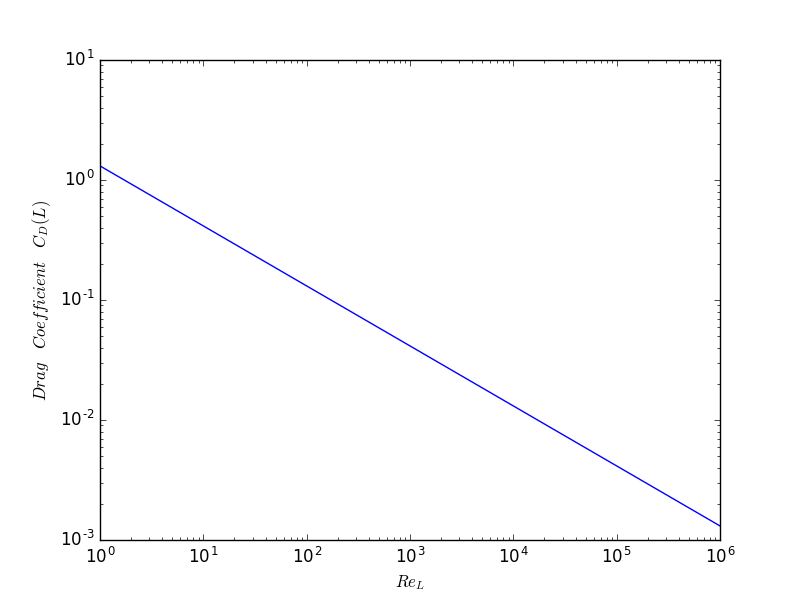
\includegraphics[width=14cm, height=12cm]{fig1.png}
    \caption{Drag of a plate}
    \label{fig:1}
\end{figure}

\end{document}
